\documentclass[11pt]{article}
\usepackage{graphicx}
\usepackage{fullpage}
\usepackage{amsmath,amsthm,amsfonts,amssymb,amscd}
\usepackage{lipsum}
\usepackage{titlesec}
\usepackage{longtable}
\usepackage[top=0.7in,bottom=1in,left=0.85in,right=0.85in]{geometry}
\usepackage[utf8]{inputenc}
\usepackage{listings}
\usepackage{xcolor}
\usepackage{verbatim}
\usepackage{setspace}

% don't indent paragraphs 
\setlength{\parindent}{0pt}
% inter-paragraph spacing
\setlength{\parskip}{1em}
% line spacing
\onehalfspacing

\definecolor{codegreen}{rgb}{0,0.6,0}
\definecolor{codegray}{rgb}{0.5,0.5,0.5}
\definecolor{codepurple}{rgb}{0.58,0,0.82}
\definecolor{backcolour}{rgb}{0.95,0.95,0.92}

\lstdefinestyle{mystyle}{
    backgroundcolor=\color{backcolour},   
    commentstyle=\color{codegreen},
    keywordstyle=\color{magenta},
    numberstyle=\tiny\color{codegray},
    stringstyle=\color{codepurple},
    basicstyle=\ttfamily\footnotesize,
    breakatwhitespace=false,         
    breaklines=true,                 
    captionpos=b,                    
    keepspaces=true,                 
    numbers=left,                    
    numbersep=5pt,                  
    showspaces=false,                
    showstringspaces=false,
    showtabs=false,                  
    tabsize=2
}
 
\lstset{style=mystyle}

% title formatting
\titleformat{\section}
{\centering\normalfont\scshape}{\thesection.}{1em}{}
\titleformat{\subsection}
{\centering\normalfont\scshape}{\thesubsection.}{1em}{}

% spacing between columns
% \setlength{\columnsep}{2em}

%title setup
\title{\vspace{-1cm}Introductory Exercise: Ohm's Law\\[0.4cm]\large{PHY224H1 S | Winter 2020}\vspace{-0.5em}}
\author{Jeff Shen}
\date{\vspace{-0.3em}\normalsize17 January 2020}

%%%%%%%%%%%%%%%%%%%%%%%%%%%%%%%%%%%
\begin{document}

\maketitle

\section{Introduction}

The setup of the circuit was as follows:
\begin{itemize}
    \item negative terminal of the power supply connected to the common terminal  of multimeter \#1
    \item ammeter terminal of multimeter \#1 connected to one side of the resistor
    \item the same side of the resistor also connected to the common terminal of multimeter \#2
    \item voltage/resistance terminal of multimeter \#2 connected to other side of the resistor
    \item the same side of the resistor also connected to the positive terminal of the power supply
\end{itemize}

\begin{figure}[htb]
    \centering 
    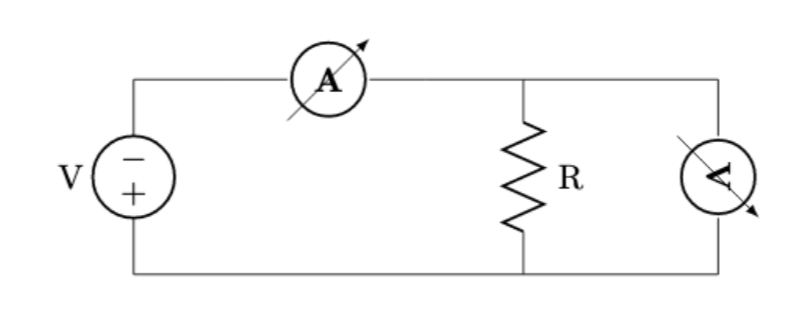
\includegraphics[width=0.5\linewidth]{circuit.png}
    \caption{\label{fig:circuit}Circuit diagram of setup.}
\end{figure}

The steps that we followed were:
\begin{enumerate}
    \item Connect setup to resistor.
    \item Turn on power supply and both multimeters.
    \item Record the voltage. 
    \item Change the voltage. 
\end{enumerate}

The lower portion of one multimeter was set to DCA (the ammeter) and the other to DCV (the voltmeter). The upper portions of the ammeter and the voltmeter were set to the lowest settings which still gave a readout (in order to get the most digits possible). In most cases, the voltmeter was at the 20V setting. We used the 2mA, 20mA, and 200mA settings on the ammeter. 

We started with the resistor that had the colour bands blue-grey-brown-gold. We performed steps 1-3 with each of the seven resistors that were available to us. Then we changed the voltage, and repeated steps 1-3. We did this a total of three times. Thus, we had three data points for each of the seven resistors. At this point, we realized that we needed to have a lot of data points for a few resistors rather than a few points for a lot of resistors. So, we conducted another round of data collection. 

We selected four resistors (blue-grey-brown-gold, green-orange-brown-gold, orange-orange-orange-gold, and grey-orange-red-gold), and for each of them, we repeated steps 3-4 a total of seven times. So, including the three data points collected earlier, we had a total of 10 data points for these four resistors. We decided not to include the data for the other three resistors. 

Afterwards, we disassembled the setup. We took one of the multimeters, and used it to measure the resistance of the three resistors that we had 10 data points for. One side of the resistor was connected to the common terminal of the multimeter, and the other to the voltage/resistance terminal. The lower portion of the multimeter was set to read the resistance. The upper portion was again, set to the lowest setting which gave us a readable output. This was the 2 kiloohm setting for the blue-grey-brown-gold and the green-orange-brown-gold resistors, the 20 kiloohm setting for the grey-orange-red-gold resistor, and the 200 kiloohm setting for the orange-orange-orange-gold resistor.

\section{Data}


\begin{table}[htb]
    \caption{\label{tab:tab1}Data for grey-orange-brown-gold resistor.}
    \vspace{1em}\hline\hline\vspace{0.3em}\centering
    \begin{tabular}{cccc}
        Current (mA)&Current Uncertainty (mA)&Voltage (V)&Voltage Uncertainty (V)\\
        \hline
1.373 mA&0.010 mA&1.122 V&0.003 V\\
3.81 mA&0.03 mA&3.11 V&0.01 V\\
6.30 mA&0.05 mA&5.12 V&0.01 V\\
6.82 mA&0.05 mA&5.53 V&0.01 V\\
9.36 mA&0.07 mA&7.60 V&0.02 V\\
9.49 mA&0.07 mA&7.72 V&0.02 V\\
14.22 mA&0.10 mA&11.56 V&0.03 V\\
15.57 mA&0.11 mA&12.67 V&0.03 V\\
17.07 mA&0.13 mA&13.83 V&0.03 V\\
19.36 mA&0.15 mA&15.64 V&0.04 V\\

    \end{tabular}
    \hline\hline
\end{table}


\begin{table}[htb]
    \caption{\label{tab:tab2}Data for orange-orange-orange-gold resistor.}
    \vspace{1em}\hline\hline\vspace{0.3em}\centering
    \begin{tabular}{cccc}
        Current (mA)&Current Uncertainty (mA)&Voltage (V)&Voltage Uncertainty (V)\\
        \hline
0.131 mA&0.001 mA&4.42 V&0.01 V\\
0.170 mA&0.001 mA&5.57 V&0.01 V\\
0.187 mA&0.001 mA&6.23 V&0.02 V\\
0.232 mA&0.002 mA&7.74 V&0.02 V\\
0.301 mA&0.002 mA&10.06 V&0.03 V\\
0.345 mA&0.003 mA&11.54 V&0.03 V\\
0.401 mA&0.003 mA&13.41 V&0.03 V\\
0.456 mA&0.003 mA&15.23 V&0.04 V\\
0.518 mA&0.004 mA&17.37 V&0.04 V\\
0.585 mA&0.004 mA&19.55 V&0.05 V\\

    \end{tabular}
    \hline\hline
\end{table}

\begin{table}[htb]
    \caption{\label{tab:tab3}Data for blue-grey-brown-gold resistor.}
    \vspace{1em}\hline\hline\vspace{0.3em}\centering
    \begin{tabular}{cccc}
        Current (mA)&Current Uncertainty (mA)&Voltage (V)&Voltage Uncertainty (V)\\
        \hline

1.96 mA&0.01 mA&1.33 V&0.01 V\\
7.34 mA&0.06 mA&4.96 V&0.01 V\\
8.22 mA&0.06 mA&5.50 V&0.01 V\\
10.77 mA&0.08 mA&7.27 V&0.02 V\\
11.50 mA&0.09 mA&7.76 V&0.02 V\\
14.35 mA&0.11 mA&9.67 V&0.02 V\\
16.89 mA&0.13 mA&11.38 V&0.03 V\\
18.55 mA&0.14 mA&12.45 V&0.03 V\\
23.8 mA&0.2 mA&15.97 V&0.04 V\\
26.2 mA&0.2 mA&17.50 V&0.04 V\\

    \end{tabular}
    \hline\hline
\end{table}


\begin{table}[htb]
    \caption{\label{tab:tab4}Data for blue-grey-brown-gold resistor.}
    \vspace{1em}\hline\hline\vspace{0.3em}\centering
    \begin{tabular}{cccc}
        Current (mA)&Current Uncertainty (mA)&Voltage (V)&Voltage Uncertainty (V)\\
        \hline

0.518 mA&0.004 mA&4.34 V&0.01 V\\
0.675 mA&0.005 mA&5.58 V&0.01 V\\
0.785 mA&0.006 mA&6.49 V&0.02 V\\
0.926 mA&0.007 mA&7.65 V&0.02 V\\
1.060 mA&0.008 mA&8.77 V&0.02 V\\
1.382 mA&0.010 mA&11.43 V&0.03 V\\
1.448 mA&0.011 mA&11.97 V&0.03 V\\
1.666 mA&0.012 mA&13.78 V&0.03 V\\
1.869 mA&0.015 mA&15.48 V&0.04 V\\
2.13 mA&0.02 mA&17.6 V&0.04 V\\

    \end{tabular}
    \hline\hline
\end{table}


\begin{table}[htb]
    \caption{\label{tab:tab5}Calculated, measured, and read resistances compared.}
    \vspace{1em}\hline\hline\vspace{0.3em}\centering
    \begin{tabular}{ccccccc}
        &Average Calculated&Standard&Measured&Measurement&Colour Band&Tolerance\\
        &Resistance&Error&Resistance&Uncertainty&Resistance&\\
        \hline
        grey-orange-&1230.45 $\Omega$&.42 $\Omega$&814 $\Omega$&2 $\Omega$&830 $\Omega$&42 $\Omega$ \\
        -brown-gold&&&&&& \\
        orange-orange-&29.96 $\Omega$&0.02 $\Omega$&33.4 $\Omega$&0.1 $\Omega$&33 $\Omega$&2 $\Omega$ \\
        -black-gold&&&&&& \\
        blue-grey-&1485.7 $\Omega$&0.7 $\Omega$&675 $\Omega$& 1 $\Omega$&680 $\Omega$&34 $\Omega$ \\
        -brown-gold&&&&&& \\
        blue-grey-&8280.14 $\Omega$&3.50 $\Omega$&8270 $\Omega$&17 $\Omega$&8300 $\Omega$&415 $\Omega$ \\
        -brown-gold&&&&&& \\
    \end{tabular}
    \hline\hline
\end{table}


\end{document}
